% COntinued Chpater Implementation
\section{Content Based Model}

The content-based model uses vector space models of a user and an item to find the similarity between two vectors. The overview of content-based model is discussed in the \autoref{fig:content_based_flowchart}. 

\begin{figure}[H]
	\centering
	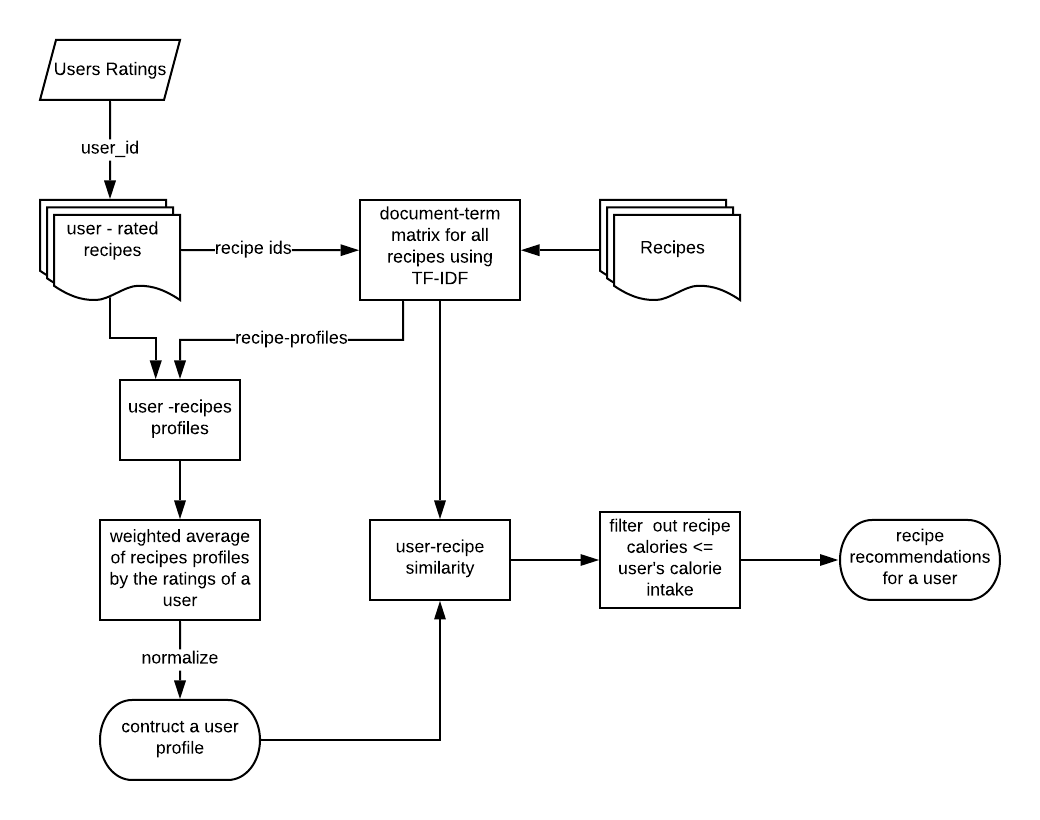
\includegraphics[width=1.0\linewidth]{content_based_flowchart}
	\caption{Content Based Filtering Flowchart }
	\label{fig:content_based_flowchart}
\end{figure}  

\noindent
All user interactions are denoted by 'Users Ratings' and all recipes information is denoted by 'Recipes'. Required steps to generated a user profile and a recipe profile are discussed below.
\begin{itemize}
\item All recipe profiles are generated based on the relevancy of terms to be considered. The term may vary based on the application area. In this thesis, ingredients, cooking methods, and diet labels are considered. The relevancy of terms in the documents is measured by TF-IDF as discussed in \nameref{sec:tf-idf}. A document term matrix is generated and stored for all recipes. 
\item Rated recipes for a single user are filtered from all user interactions.
Rated recipes are then filtered out and stored from a stored document-term matrix. 
\item To construct a user profile, recipes vectors rated by a user are considered. Then a weighted average of rated recipe profiles is calculated. The user profile is further normalized on the weighted values. 
\item Similarity between the user profile and all recipe profiles from the dataset is measured by cosine similarity as discussed in \nameref{cosine_similarity}. Recipes that are rated previously by the user are omitted to calculate relevance. Sort these recipes in descending order of similarity scores.
\item On the resultant recipes vectors we have applied a calorie intake filter comparing recipe calories and user required calories. These recipes are offered as recommendations to the user.  
\end{itemize}
 

\subsection{Recommendations Using Ingredients}
\subsection{Recommendations Using Ingredients and Cooking Methods}
\subsection{Recommendations Using Ingredients, Cooking Method and Diet Labels}
\section{Collaborative Filtering Model}
\section{Hybrid Filtering Model(CB and CF)}